\section{Discussion and Analysis}

In this section we discuss our results and compare them to the human score. We elaborate on potential limiting factors, capping the maximum achievable accuracy. Furthermore, we analyze the model internals and try to interpret them.

\subsection{Accuracy}

The page rank estimation task is difficult. Our model is provided with screenshots of up to eight webpages of a domain as well as their link structure. Given two samples of that kind, guessing the relative ranking is hard. In the real world, a website's popularity depends on many factors other than its look. By achieving accuracies significantly beyond random guessing (50\%), we do however show that a website's look correlates to some extent with its rank. Obviously, a deduction on the causal relationship between look and rank would be purely speculative.

The human score gives an idea of the performance of our model. Even though the model achieves super-human results, it seems unlikely that more sophisticated methods can push the accuracy much further to, say, 90\%. We suspect the upper limit of purely vision-based rank estimation to be below 70\%.

Another aspect of difficulty is noise in the dataset: When crawling and screenshotting 100k websites, some errors are almost inevitable. A small but not negligible percentage of our data is therefore corrupt, e.g. because the website has not finished loading by the time we took the screenshot. Consequently, our model is confronted with all- or almost all-black screenshots occasionally.

It is noteworthy that the dataset size was sufficient to prevent our CNN architecture from overfitting. We saw no need to make use of regularization methods such as weight decay or data augmentation because the accuracy on training and validation data was almost the same throughout all training runs. We therefore suspect that a model with greater capacity might be able to capture more fine-grained details of screenshots, thereby achieving a higher accuracy.

The accuracy score as proposed in Equation \ref{eq:acc} has some \textit{unfairness} to it because the distance of two compared samples is disregarded. For example, a erroneous assessment of the relative ranking of two samples with ranks \#12,000 and \#12,001 is contributing to the accuracy just like the confusion of samples with ranks \#1,000 and \#25,000, even though the latter should be easier to disentangle. An alternative formulation could take the difficulty of a pairwise comparison into account.

In summary, we can strongly assume that a correlation between page rank and visual features exists. Our model was able to learn these features and make use of them to solve the pairwise ranking task with an accuracy of xx.x\%. Based on the assumption that an upper limit below 70\% exists, which cannot be exceeded by purely vision-based models, the outcomes of our trainings are a success.

\subsection{Model Understanding}

Besides ranking websites our model has the practical purpose of yielding interpretable information. In this section we try to understand the model internals and deduce practical information from them. While it is a common method to look at the kernels of CNNs (see e.g. Figure 3 of \cite{krizhevsky:imagenet}), this approach is not reasonably applicable to our architecture because our filter tensors have a spatial dimension of at most $3\times3$. Instead, we analyze the CNN feature maps, retrieve hard and easy samples, and compute the gradient of the output with respect to the input.

A qualitative analysis of the feature maps suggests that the model learns to discriminate different elements of webpages such as natural images or text. We have observed some filters to get excited by layout elements such as edges and corners. Figure \ref{fig:activationmaps} shows some cherry-picked filters from all layers.

Instead, we analyze the \textbf{activation maps} our model. Activation maps are internal representations (latent variables) of the input at intermediate stages of the model. Specifically, we consider the input, features before pooling and the last ReLU activation of Block1, Block2, Block3, and Block4. The sizes of these tensors are listed in Table \ref{tab:activationmaptensors}.

\begin{table}
    \centering
    \begin{tabular}{lrr}
        \textbf{Feature map} & \textbf{Spatial size (desktop, mobile)} & \textbf{Depth}\\\hline
        \textbf{Input} & $480\times270\mid480\times270$ & $3$\\
        \textbf{Block1} & $480\times270$ & $3$\\
        \textbf{Block2} & $480\times270$ & $3$\\
        \textbf{Block3} & $480\times270$ & $3$\\
        \textbf{Block4} & $480\times270$ & $3$\\
    \end{tabular}
    \caption[Comparison of GN variants]{Comparison of GN variants}
    \label{tab:activationmaptensors}
\end{table}

\begin{figure}
    \centering
    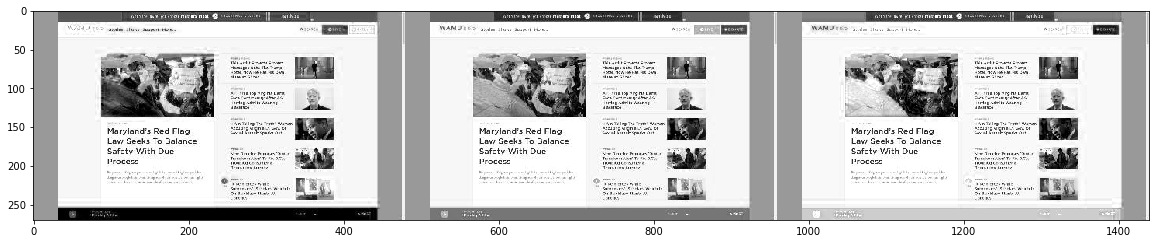
\includegraphics[clip,width=\columnwidth]{resources/analysis/feat-map-0.png}\\
    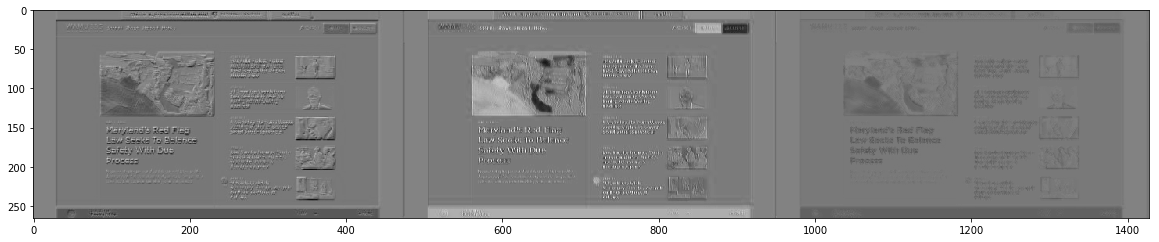
\includegraphics[clip,width=\columnwidth]{resources/analysis/feat-map-1.png}\\
    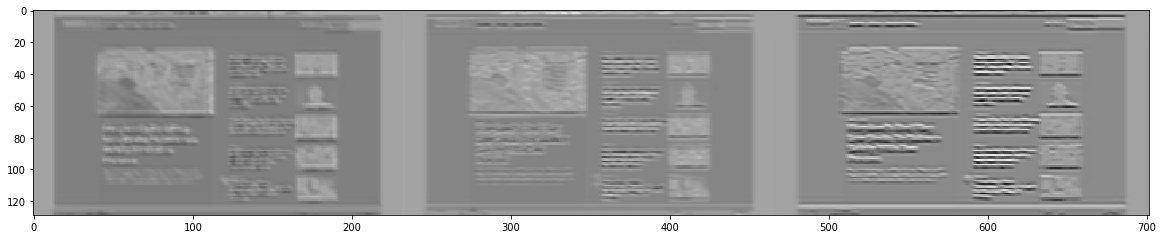
\includegraphics[clip,width=\columnwidth]{resources/analysis/feat-map-2.png}\\
    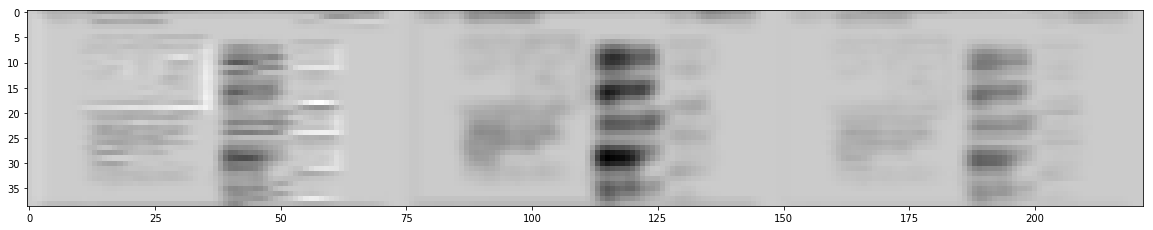
\includegraphics[clip,width=\columnwidth]{resources/analysis/feat-map-3.png}\\
    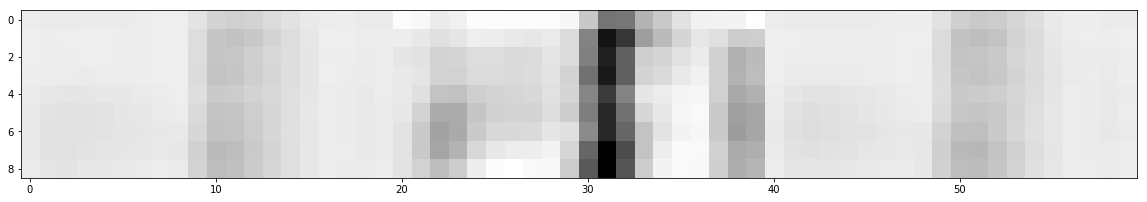
\includegraphics[clip,width=\columnwidth]{resources/analysis/feat-map-4.png}\\
    \caption[Activation maps of the CNN]{Activation maps of the CNN. Top to bottom: Input, Block1, Block2, Block3, and Block4.}
    \label{fig:activationmaps}
\end{figure}

We introduce the notion of \textbf{hard and easy samples}. A hard sample from the dataset is characterized by the property that a given model's estimation of its rank diverges significantly from its actual rank. This can be quantized by evaluating Equation \ref{eq:inference} (inference) and comparing the inferred rank with the ground-truth rank. Samples for which the difference is large are considered hard, because the model has trouble estimating their rank properly. Easy samples are the opposite: Relative to the other samples in the dataset, the model is capable of predicting the correct ranking relatively often.

Hard and easy samples have qualitative meaning because they are representative for websites of their particular rank: Give for instance an easy sample with a high rank, it can be assumed that this sample is representative for high ranked websites. A hard sample with a high rank might have attained its rank for reasons other than its look. On the other hand, easy samples with low rank are representative for websites with a low rank. By comparing easy samples with high/low rank we can distill the visual difference between high and low ranked websites. Note that this is more sophisticated than looking only at the pure dataset, i.e. comparing high-ranked samples with low-ranked samples, because the model acts as a filter, extracting the visually representative samples.

In the following, we set the easiness threshold to xx\%. A sample is considered easy if it has been ranked correctly with respect to at least xx\% of the remainder of the dataset.

\begin{figure}
    \centering
    % include graphics
    \caption[Easy samples across all ranks]{Easy samples across all ranks, xxx...}
    \label{fig:easysamples}
\end{figure}

\begin{figure}
    \centering
    % include graphics
    \caption[Hard samples across all ranks]{Hard samples across all ranks, xxx...}
    \label{fig:hardsamples}
\end{figure}

Our last model analysis method is the computation of the \textbf{gradient $\tensorsym{G}$ of the model output with respect to the input}. It highlights areas, which when changed, have strong influence on the assessment of the given sample. The mathematical formulation is\begin{equation}
    \tensorsym{G}=\frac{\partial f\left(\tensorsym{I}\right)}{\partial\tensorsym{I}}\,,
\end{equation}where $\tensorsym{I}$ can be either a desktop or a mobile image. In the following, the function $f$ is a screenshot feature extractor without graph network. To ensure the gradient is meaningful, we chose a samples which the model classifies with high accuracy, i.e. easy ones.

Figure \ref{fig:gradwrtinput} shows $\tensorsym{G}$ for an easy sample. Interpretation xxx.

\begin{figure}
    \centering
    % include graphics
    \caption[Areas with high influence on the model prediction]{Areas with high influence on the model prediction, xxx...}
    \label{fig:gradwrtinput}
\end{figure}
